In order to calculate the probability for the Markov chain we decided to choose a Gaussian Distribution for our probability density function. In probability theory, the normal (or Gaussian) distribution is a very commonly occurring continuous probability distribution, which is a function that tells the probability that any real observation will fall between any two real limits or real numbers, as the curve approaches zero on either side. In our case we want to consider the distribution only in the positive interval of x axes. The equation for the normal distribution is:

\begin{center}
\begin{equation}
\phi (x,\sigma,\mu) = 	\begin{cases}
							1 & x < \mu \\
							e^{-\frac{(x-\mu )^2}{2 \sigma ^2}} & x \geq \mu
						\end{cases}
\end{equation}

\end{center}
~\\
Where $\sigma$ is the standard deviation and $\mu$ is the mean. With these two parameters, it is possible to tune our function for different scenarios. For example to decide when an SCV should go building a new Supply Depot or going back harvesting as well as to decide when to build a new unit. 

Figure \ref{fig:gaussdistr} shows the distribution plotted with the aid of a computational software called \textit{Mathematica}. We picked to random values for mean and standard deviation, but those two will be tuned accordingly to a specific event that the markov chain will represent.

\begin{figure}[h]
\caption{Gaussian Distribution}
\centering
\label{fig:gaussdistr}
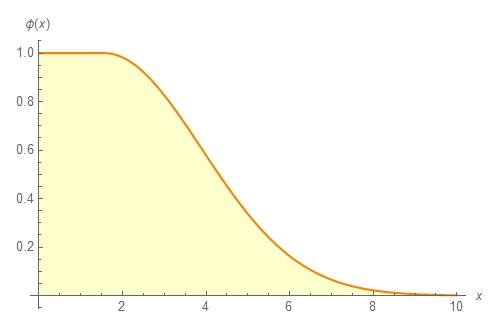
\includegraphics[scale=0.7]{images/Gaussian_Distribution.jpg}
\end{figure}
